\documentclass[11pt]{article}
\usepackage[a4paper,margin=1in]{geometry}
\usepackage{amsmath,amssymb,amsthm}
\usepackage{booktabs}
\usepackage{tikz}
\usepackage{siunitx}
\usepackage[hidelinks]{hyperref}
\usepackage{enumitem}

\newtheorem{assumption}{Assumption}
\newtheorem{remark}{Remark}

\title{\textbf{Guaranteed-Collision Reachability for a Twin-Thruster\\
Autonomous Surface Vessel: a Two-Player\\
Hamilton--Jacobi--Isaacs Formulation}}
\author{Shailesh Yadav\\
\small MAVLab, Department of Ocean Engineering, IIT Madras\\
\small Advisor: Prof.\ Abhilash Somayajula}
\date{\today}

\newcommand{\R}{\mathbb{R}}
\newcommand{\zvec}{\boldsymbol{\zeta}}
\newcommand{\nuv}{\boldsymbol{\nu}}
\newcommand{\pvec}{\boldsymbol{p}}

\begin{document}
\pagestyle{plain}
\maketitle

\begin{abstract}
This document sets out the complete mathematical methodology for computing the
region of guaranteed collision (the \emph{danger} set) and its complement (the
\emph{safe} set) for two identical twin-thruster autonomous surface vessels
(ASVs) approaching head-on. Both vessels obey full three-degree-of-freedom
Fossen dynamics with an experimentally identified hydrodynamic damping model.
The interaction is posed as a zero-sum pursuit--evasion differential game: a
pursuer that drives toward collision and an evader that avoids it. The game value
is the unique viscosity solution of a Hamilton--Jacobi--Isaacs (HJI) variational
inequality, whose zero sub-level set is the backward reachable tube (BRT) of the
collision set. Because the two thruster forces enter the dynamics separately and
each actuator set is a convex ellipse, the Hamiltonian admits a closed form and
the game value exists. The value function is represented by a physics-informed
neural network (PINN) with an exact terminal-condition ansatz. All numerical
parameters are those of the vessel \emph{Sookshma}. A layered verification plan is
included.
\end{abstract}

\tableofcontents

%======================================================================
\section{Problem setting}
Two identical ASVs operate in the horizontal plane: a \emph{pursuer} (subscript
$i$) and an \emph{evader} (subscript $e$). The pursuer seeks to reduce the
inter-vessel separation below a collision radius $R>0$; the evader seeks to keep
it above $R$. Each vessel is actuated by two fixed, parallel, forward-only
thrusters. We treat this as a single, two-player, zero-sum differential game and
compute the set of relative states from which collision is unavoidable under the
evader's best avoidance and the pursuer's best pursuit. This is a
Hamilton--Jacobi--Isaacs reachability problem, solved here with a
physics-informed neural network.

%======================================================================
\section{Vessel dynamics: three-degree-of-freedom Fossen model}
With body-frame velocity $\nuv=(u,v,r)^{\top}$ (surge, sway, yaw-rate) and
generalised force $\boldsymbol{\tau}=(\tau_u,0,\tau_r)^{\top}$, each vessel obeys
the standard manoeuvring model
\begin{equation}
\mathbf{M}\dot{\nuv} + \mathbf{C}(\nuv)\nuv + \mathbf{D}(\nuv)\nuv
= \boldsymbol{\tau},
\qquad
\dot{\nuv}=\mathbf{M}^{-1}\!\left[\boldsymbol{\tau}
-\mathbf{C}(\nuv)\nuv-\mathbf{D}(\nuv)\nuv\right].
\label{eq:fossen}
\end{equation}
The sway force is identically zero because the two parallel thrusters produce only
surge force and yaw moment.

\begin{assumption}[Hull symmetry]
The body origin is at the centre of gravity and the vessel has port--starboard
symmetry, so the mass matrix is diagonal:
\begin{equation}
\mathbf{M}=\mathrm{diag}(M_{11},M_{22},M_{33}),\quad
M_{11}=m-X_{\dot u},\;
M_{22}=m-Y_{\dot v},\;
M_{33}=I_z-N_{\dot r}.
\end{equation}
\end{assumption}

\noindent
Under this assumption the Coriolis--centripetal matrix and the scalar equations of
motion are
\begin{equation}
\mathbf{C}(\nuv)=
\begin{pmatrix}
0 & 0 & -M_{22}v\\
0 & 0 & M_{11}u\\
M_{22}v & -M_{11}u & 0
\end{pmatrix},
\end{equation}
\begin{align}
\dot u &= \tfrac{1}{M_{11}}\big[\tau_u + M_{22}\,v\,r - X_D(u,v,r)\big],\label{eq:udot}\\
\dot v &= \tfrac{1}{M_{22}}\big[-M_{11}\,u\,r - Y_D(u,v,r)\big],\label{eq:vdot}\\
\dot r &= \tfrac{1}{M_{33}}\big[\tau_r + (M_{11}-M_{22})\,u\,v - N_D(u,v,r)\big].\label{eq:rdot}
\end{align}

\subsection{Identified damping model}
The hydrodynamic damping vector $\mathbf{D}(\nuv)\nuv=(X_D,Y_D,N_D)^{\top}$ is an
experimentally identified polynomial in $(u,v,r)$, replacing the classical linear
plus quadratic diagonal form. Its regressor structure respects port--starboard
symmetry (surge even in $v,r$; sway and yaw odd):
\begin{align}
X_D &= D^{x}_{u}u + D^{x}_{u^2}u^2 + D^{x}_{v^2}v^2 + D^{x}_{r^2}r^2
     + D^{x}_{vr}vr + D^{x}_{u^3}u^3 \nonumber\\
    &\quad + D^{x}_{uv^2}uv^2 + D^{x}_{ur^2}ur^2 + D^{x}_{uvr}uvr + D^{x}_{|u|u}|u|u,\\
Y_D &= D^{y}_{v}v + D^{y}_{r}r + D^{y}_{uv}uv + D^{y}_{ur}ur + D^{y}_{v^3}v^3
     + D^{y}_{r^3}r^3 \nonumber\\
    &\quad + D^{y}_{u^2v}u^2v + D^{y}_{u^2r}u^2r + D^{y}_{v^2r}v^2r
     + D^{y}_{vr^2}vr^2 + D^{y}_{|v|v}|v|v + D^{y}_{u|v|}u|v|,\\
N_D &= D^{n}_{v}v + D^{n}_{r}r + D^{n}_{uv}uv + D^{n}_{ur}ur + D^{n}_{v^3}v^3
     + D^{n}_{r^3}r^3 \nonumber\\
    &\quad + D^{n}_{u^2v}u^2v + D^{n}_{u^2r}u^2r + D^{n}_{v^2r}v^2r
     + D^{n}_{vr^2}vr^2 + D^{n}_{|r|r}|r|r + D^{n}_{u|r|}u|r|.
\end{align}
The $34$ coefficients (set ``$\theta_{\mathrm{anneal}}$'') are dimensional and
identical for both vessels; they are listed with the model files.

\subsection{Added mass from non-dimensional derivatives}
The added-mass derivatives are supplied in non-dimensional (prime-system) form and
converted to physical units using water density $\rho$ and vessel length $L$; added
mass is a pure inertia and carries no dependence on forward speed:
\begin{equation}
X_{\dot u}=X'_{\dot u}\tfrac12\rho L^3,\quad
Y_{\dot v}=Y'_{\dot v}\tfrac12\rho L^3,\quad
N_{\dot r}=N'_{\dot r}\tfrac12\rho L^5 .
\end{equation}
Sway--yaw cross terms ($Y_{\dot r},N_{\dot v}$) are available but set to zero here,
keeping $\mathbf{M}$ diagonal.

%======================================================================
\section{The nine-dimensional relative state}
Working in the pursuer body frame, define
\begin{equation}
\zvec=(X,\,Y,\,\psi_{\mathrm{rel}},\,u_e,\,v_e,\,u_i,\,v_i,\,r_e,\,r_i)^{\top}\in\R^{9},
\end{equation}
where $(X,Y)$ is the evader position relative to the pursuer and
$\psi_{\mathrm{rel}}=\psi_e-\psi_i$ the relative heading. The relative kinematics
are
\begin{align}
\dot X &= u_e\cos\psi_{\mathrm{rel}} - v_e\sin\psi_{\mathrm{rel}} - u_i + r_i Y,\\
\dot Y &= u_e\sin\psi_{\mathrm{rel}} + v_e\cos\psi_{\mathrm{rel}} - v_i - r_i X,\\
\dot\psi_{\mathrm{rel}} &= r_e - r_i,
\end{align}
and the six velocity components follow each vessel's dynamics
\eqref{eq:udot}--\eqref{eq:rdot}. The head-on encounter is the slice
$\psi_{\mathrm{rel}}=\pi$ with both vessels closing.

\begin{center}
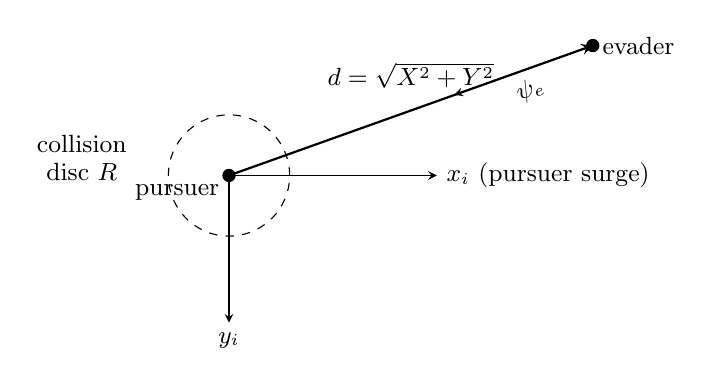
\begin{tikzpicture}[>=stealth,scale=1.1]
  \draw[->] (0,0) -- (2.4,0) node[right]{\small $x_i$ (pursuer surge)};
  \draw[->] (0,0) -- (0,-1.7) node[below]{\small $y_i$};
  \draw[dashed] (0,0) circle (0.7cm);
  \node[align=center] at (-1.7,0.2) {\small collision\\[-2pt]\small disc $R$};
  \filldraw (0,0) circle (2pt) node[below left]{\small pursuer};
  \draw[->,thick] (0,0) -- (4.2,1.5);
  \node at (2.1,1.15) {\small $d=\sqrt{X^2+Y^2}$};
  \filldraw (4.2,1.5) circle (2pt) node[right]{\small evader};
  \draw[->] (4.2,1.5) -- (2.6,0.93) node[midway,below,sloped]{\small $\psi_e$};
\end{tikzpicture}
\end{center}

%======================================================================
\section{Control-affine form and actuator model}
Substituting each vessel's dynamics, the system is control-affine in the two
thruster commands $\mathbf{u}_i=(\tau_u^i,\tau_r^i)$ and
$\mathbf{u}_e=(\tau_u^e,\tau_r^e)$:
\begin{equation}
\dot{\zvec}= \mathbf{a}_0(\zvec) + \mathbf{G}_i\,\mathbf{u}_i + \mathbf{G}_e\,\mathbf{u}_e ,
\end{equation}
where $\mathbf{a}_0$ is the drift (relative kinematics plus the control-independent
part of both vessels' dynamics), and each input matrix injects thrust only into
its own surge and yaw-rate rows,
$\mathbf{G}_\bullet$ having non-zero entries $1/M_{11}$ and $1/M_{33}$.

\subsection{Ellipsoidal thruster set}
Each thruster force satisfies $F_p,F_s\in[0,F_{\max}]$, with allocation
$\tau_u=F_p+F_s$, $\tau_r=d(F_s-F_p)$ ($d$ the thruster arm). The reachable
$(\tau_u,\tau_r)$ region is a diamond; we use its largest inscribed ellipse
(a smooth, conservative inner approximation) centred at $(F_{\max},0)$ with
semi-axes
\begin{equation}
\alpha_u=\frac{F_{\max}}{\sqrt2},\qquad
\alpha_r=\frac{d\,F_{\max}}{\sqrt2},\qquad
\boldsymbol{\Sigma}=\mathrm{diag}(\alpha_u^2,\alpha_r^2).
\end{equation}

%======================================================================
\section{Collision set, value function, and the danger/safe sets}
The signed distance to the collision disc and the collision (target) set are
\begin{equation}
\ell(\zvec)=\sqrt{X^2+Y^2}-R,\qquad
\mathcal{L}=\{\zvec:\ell(\zvec)\le 0\}.
\end{equation}
The value function is the backward reachable \emph{tube} of $\mathcal{L}$,
\begin{equation}
V(\zvec,t)=\min_{\mathbf{u}_i(\cdot)}\;\max_{\mathbf{u}_e(\cdot)}\;
\min_{s\in[t,0]}\;\ell\big(\zvec(s)\big),
\label{eq:value}
\end{equation}
i.e.\ the pursuer minimises the closest approach and the evader maximises it. Its
sign partitions the state space:
\begin{equation}
\underbrace{\{\zvec:V\le0\}}_{\text{DANGER (collision unavoidable)}},
\qquad
\underbrace{\{\zvec:V>0\}}_{\text{SAFE}},
\qquad
\underbrace{\{\zvec:V=0\}}_{\text{barrier}} .
\end{equation}
Because the two controls act on disjoint costate components and each actuator set is
convex, the Isaacs condition holds ($\min\max=\max\min$) and the game value
\eqref{eq:value} is well defined.

%======================================================================
\section{Isaacs Hamiltonian and optimal controls}
Let $\pvec=\nabla_{\zvec}V$ be the costate and define the costate directions
$c_0^{i}=p_{u_i}/M_{11}$, $c_1^{i}=p_{r_i}/M_{33}$ (and likewise $c_0^{e},c_1^{e}$
for the evader). The optimal Hamiltonian is
\begin{equation}
H(\zvec,\pvec)=\min_{\mathbf{u}_i\in\mathcal{E}}\;\max_{\mathbf{u}_e\in\mathcal{E}}\;
\pvec^{\top}\!\big(\mathbf{a}_0+\mathbf{G}_i\mathbf{u}_i+\mathbf{G}_e\mathbf{u}_e\big),
\end{equation}
which, using the ellipse support function, has the closed form
\begin{equation}
\boxed{\;
H(\zvec,\pvec)=\pvec^{\top}\mathbf{a}_0(\zvec)
+\big[F_{\max}c_0^{i}-\mathcal{R}_i\big]
+\big[F_{\max}c_0^{e}+\mathcal{R}_e\big],\quad
\mathcal{R}_\bullet=\sqrt{\alpha_u^2 (c_0^\bullet)^2+\alpha_r^2 (c_1^\bullet)^2+\varepsilon}\; }
\end{equation}
The pursuer term carries $-\mathcal{R}_i$ (minimisation) and the evader term
$+\mathcal{R}_e$ (maximisation); $\varepsilon\sim10^{-6}$ rounds the norm corner.
The saddle-point controls are
\begin{equation}
\mathbf{u}_i^{\ast}=\Big(F_{\max}-\tfrac{\alpha_u^2 c_0^{i}}{\mathcal{R}_i},\,
-\tfrac{\alpha_r^2 c_1^{i}}{\mathcal{R}_i}\Big),\qquad
\mathbf{u}_e^{\ast}=\Big(F_{\max}+\tfrac{\alpha_u^2 c_0^{e}}{\mathcal{R}_e},\,
+\tfrac{\alpha_r^2 c_1^{e}}{\mathcal{R}_e}\Big),
\end{equation}
both of which lie inside the physical thruster diamond.

%======================================================================
\section{Hamilton--Jacobi--Isaacs variational inequality}
The value function is the unique viscosity solution, on $t\in[-T,0]$, of
\begin{equation}
\boxed{\;
\min\Big\{\;\frac{\partial V}{\partial t}+H(\zvec,\nabla_{\zvec}V),\;\;
\ell(\zvec)-V\;\Big\}=0,\qquad V(\zvec,0)=\ell(\zvec).\;}
\label{eq:hjivi}
\end{equation}
The term $\min\{\,\cdot\,,\ell-V\}$ enforces the tube semantics: once the trajectory
enters $\mathcal{L}$ it is counted as captured for all remaining time.

%======================================================================
\section{Physics-informed neural-network solution}
The value is represented by a sinusoidal-activation network
$N_\theta(\zvec,t)$ with the relative heading encoded as $(\cos\psi_{\mathrm{rel}},
\sin\psi_{\mathrm{rel}})$ so periodicity holds by construction. An exact
boundary-condition ansatz is used:
\begin{equation}
V_\theta(\zvec,t)=\ell(\zvec)+t\,\operatorname{softplus}\!\big(N_\theta(\zvec,t)\big),
\end{equation}
which makes the terminal condition $V_\theta(\zvec,0)=\ell(\zvec)$ exact and the
tube property $V_\theta\le\ell$ hold for all $t\le0$ automatically. Training
minimises the mean-squared residual of \eqref{eq:hjivi} over collocation points
sampled in $\R^9\times[-T,0]$,
\begin{equation}
\mathcal{J}(\theta)=\mathbb{E}_{\zvec,t}\!\left[\Big(
\min\{\partial_t V_\theta+H(\zvec,\nabla_{\zvec}V_\theta),\;\ell-V_\theta\}\Big)^2\right],
\end{equation}
with the costate $\nabla_{\zvec}V_\theta$ obtained by automatic differentiation and a
backward-in-time curriculum that grows the horizon from $0$ to $T$.

%======================================================================
\section{Numerical parameters (\emph{Sookshma})}
\begin{center}
\begin{tabular}{@{}llll@{}}
\toprule
Quantity & Symbol & Value & Unit\\
\midrule
Mass & $m$ & $20.0$ & \si{kg}\\
Yaw inertia & $I_z$ & $1.88$ & \si{kg.m^2}\\
Surge added mass & $X_{\dot u}$ & $-1.72$ & \si{kg}\\
Sway added mass & $Y_{\dot v}$ & $-9.214$ & \si{kg}\\
Yaw added inertia & $N_{\dot r}$ & $-0.4232$ & \si{kg.m^2}\\
Effective mass matrix & $\mathbf{M}$ & $\mathrm{diag}(21.72,\,29.214,\,2.3032)$ & --\\
Thruster arm & $d$ & $0.20$ & \si{m}\\
Max thruster force & $F_{\max}$ & $17.85$ ($=1.82$\,kgf) & \si{N}\\
Surge authority & $\tau_{u,\max}=2F_{\max}$ & $35.70$ & \si{N}\\
Yaw authority & $\tau_{r,\max}=dF_{\max}$ & $3.57$ & \si{N.m}\\
Ellipse semi-axes & $(\alpha_u,\alpha_r)$ & $(12.62,\,2.52)$ & --\\
Collision radius & $R$ & $1.0$ & \si{m}\\
Horizon & $T$ & $20$ & \si{s}\\
Water density & $\rho$ & $1000$ & \si{kg/m^3}\\
Reference length & $L$ & $1.0$ & \si{m}\\
\bottomrule
\end{tabular}
\end{center}

%======================================================================
\section{Verification methodology}
Correctness is established in layers.
\begin{description}[leftmargin=1.4em]
\item[(a) Implementation faithfulness.] Automated checks confirm the code
computes the stated equations: equilibrium ($\dot\nuv=0$ at rest), the
Coriolis term is workless ($\nuv^{\top}\mathbf{C}(\nuv)\nuv=0$), port--starboard
symmetry (symmetric thrust keeps sway and yaw exactly zero), fourth-order
Runge--Kutta convergence against a reference integrator, and energy dissipation
under free decay. For the game, the closed-form Hamiltonian is checked against a
brute-force minimisation--maximisation over the ellipses, the Isaacs gap
$|\!\min\max-\max\min|$ is confirmed zero, and the saddle controls are shown
realisable. Network gradients are checked against finite differences.
\item[(b) Training convergence.] The residual $\mathcal{J}(\theta)$ must fall and
stabilise, and the barrier $\{V=0\}$ must stop moving between checkpoints.
\item[(c) Reachability sanity.] As $T\to0$ the danger set must collapse to the
disc; it must grow monotonically with $T$; it must be symmetric under $Y\to-Y$ for
the symmetric head-on case; and it must enlarge with closing speed.
\item[(d) Closed-loop rollout (primary test).] From many initial states, integrate
the game with both saddle-point controls and record the realised minimum
separation; the states with minimum separation $\le R$ must coincide with
$\{V\le0\}$. A Monte-Carlo sweep yields a quantitative false-safe / false-danger
rate.
\item[(e) Independent reference.] A grid-based Hamilton--Jacobi level-set solve on
a reduced-dimension version cross-validates the network barrier.
\item[(f) Model validity.] The identified dynamics are validated against logged
sea-trial trajectories via one-step acceleration error (root-mean-square error per
axis) and multi-step track overlay; the reachability result is exact only for the
assumed model.
\end{description}

\begin{remark}[Scope of the guarantee]
The barrier certifies capturability of the specific game defined above (both
vessels optimal, identical actuator limits). It is not a claim of robustness to an
arbitrary threat with different capability; asymmetric limits would enter through
distinct $\mathbf{G}_i,\mathbf{G}_e$.
\end{remark}

\begin{thebibliography}{9}
\bibitem{fossen} T.\,I.\ Fossen, \emph{Handbook of Marine Craft Hydrodynamics and
Motion Control}, Wiley, 2011.
\bibitem{mitchell} I.\ Mitchell, A.\ Bayen, C.\ Tomlin, ``A time-dependent
Hamilton--Jacobi formulation of reachable sets for continuous dynamic games,''
\emph{IEEE TAC}, 2005.
\bibitem{bansal} S.\ Bansal, M.\ Chen, S.\ Herbert, C.\ Tomlin, ``Hamilton--Jacobi
reachability: a brief overview and recent advances,'' \emph{IEEE CDC}, 2017.
\bibitem{deepreach} S.\ Bansal, C.\ Tomlin, ``DeepReach: a deep learning approach
to high-dimensional reachability,'' \emph{IEEE ICRA}, 2021.
\bibitem{siren} V.\ Sitzmann et al., ``Implicit neural representations with
periodic activation functions (SIREN),'' \emph{NeurIPS}, 2020.
\end{thebibliography}

\end{document}
